\chapter{Linear and Logistic Regression}

\begin{ex}
  Recall that the least squares estimates are the values $\betahat_0$ and
  $\betahat_1$ that minimize
  $\textsc{rss}=\sum_{i=1}^n(Y_i-\betahat_1X_i-\betahat_0)^2$. This is a
  quadratic function with positive leading coefficients in both $\betahat_1$ and
  $\betahat_0$, and therefore will achieve its minimum at a critical point. To
  that end, we take partial derivatives with respect to $\betahat_1$ and
  $\betahat_1$, set them equal to zero and solve.
  \begin{align*}
    0 & =\frac{\pd{\textsc{RSS}}}{\pd \betahat_0}    \\
      & =2\sum_{i=1}^n(Y_i-\betahat_1X_i-\betahat_0) \\
      & =2n(\Ybar-\betahat_1\Xbar-\betahat_0),
  \end{align*}
  and therefore,
  \[
    \betahat_0 = \Ybar-\betahat_1\Xbar.
  \]

  Hence,
  \begin{align*}
    0 & =\frac{\pd{\textsc{RSS}}}{\pd \betahat_1}               \\
      & =-2\sum_{i=1}^nX_i(Y_i-\betahat_1X_i-\betahat_0)        \\
      & =-2\left(\sum_{i=1}^nX_iY_i-\betahat_1\sum_{i=1}^nX^2_i
    +n\betahat_1\Xbar^2-n\Xbar\Ybar\right),
  \end{align*}
  or,
  \[
    \betahat_1=\frac{\sum_{i=1}^nX_iY_i-n\Xbar\Ybar}{\sum_{i=1}^nX_i^2-n\Xbar^2}.
  \]

  Since
  \begin{align*}
    \sum_{i=1}^nX_iY_i-n\Xbar\Ybar
     & =\sum_{i=1}^n\left(X_iY_i-\Xbar\Ybar\right)                       \\
     & =\sum_{i=1}^n\left(X_iY_i-\Xbar\Ybar-\Xbar\Ybar+\Xbar\Ybar\right) \\
     & =\sum_{i=1}^n\left(X_iY_i-X_i\Ybar-\Xbar Y_i+\Xbar\Ybar\right)    \\
     & =\sum_{i=1}^n\left(X_i(Y_i-\Ybar)-\Xbar(Y_i-\Ybar)\right)         \\
     & =\sum_{i=1}^n(X_i-\Xbar)(Y_i-\Ybar),
  \end{align*}
  and
  \begin{align*}
    \sum_{i=1}^nX_i^2-n\Xbar^2
     & =\sum_{i=1}^n\left(X_i^2-\Xbar^2\right)           \\
     & =\sum_{i=1}^n\left(X_i^2-2\Xbar^2+\Xbar^2\right)  \\
     & =\sum_{i=1}^n\left(X_i^2-2X_i\Xbar+\Xbar^2\right) \\
     & =\sum_{i=1}^n\left(X_i-\Xbar\right)^2,
  \end{align*}
  it follows that
  \[
    \betahat_1
    =\frac{\sum_{i=1}^n(X_i-\Xbar)(Y_i-\Ybar)}{\sum_{i=1}^n\left(X_i-\Xbar\right)^2}.
  \]

  Note that
  \begin{align*}
    \widehat{\epsilon}_i
     & =Y_i-\Yhat_i                                                             \\
     & =\beta_1X_i+\beta_0+\epsilon_i
    -\betahat_1X_i-\betahat_0                                                   \\
     & =\beta_1X_i+\beta_0+\epsilon_i
    -\betahat_1X_i+\betahat_1\Xbar-\Ybar                                        \\
     & =(\epsilon_i+\beta_1\Xbar+\beta_0-\Ybar)-(\betahat_1-\beta_1)(X_i-\Xbar) \\
     & =(\epsilon_i-\epsbar)-(\betahat_1-\beta_1)(X_i-\Xbar),
  \end{align*}
  since
  \begin{align*}
    \beta_1\Xbar+\beta_0-\Ybar
     & =\beta_1\left(\sum_{i=1}^nX_i\right)+\beta_0-\sum_{i=1}^n Y_i                                                   \\
     & =\frac{\beta_1}{n}\left(\sum_{i=1}^n X_i\right)+\beta_0-\frac{1}{n}\sum_{i=1}^n (\beta_1X_i+\beta_0+\epsilon_i) \\
     & =-\frac{1}{n}\sum_{i=1}^n\epsilon_i.
  \end{align*}

  Therefore,
  \begin{align*}
    \var{\widehat{\epsilon}_i}
     & =\var{(\epsilon_i-\epsbar)-(\betahat_1-\beta_1)(X_i-\Xbar)}     \\
     & =\var{\epsilon_i-\epsbar}+\var{(\betahat_1-\beta_1)(X_i-\Xbar)}
    -2\cov{\epsilon_i-\epsbar, (\betahat_1-\beta_1)(X_i-\Xbar)}        \\
     & =\var{\epsilon_i-\epsbar}+(X_i-\Xbar)^2\var{\betahat_1-\beta_1}
    -2(X_i-\Xbar)\cov{\epsilon_i-\epsbar, \betahat_1-\beta_1},
  \end{align*}
  where
  \begin{align*}
    \var{\epsilon_i-\epsbar}
     & =\var{\epsilon_i}+\var{\epsbar}-2\cov{\epsilon_i,\epsbar}   \\
     & =\var{\epsilon_i}+\frac{1}{n^2}\var{\sum_{j=1}^n\epsilon_j}
    -\frac{2}{n}\cov{\epsilon_i,\sum_{j=1}^n\epsilon_j}            \\
     & =\sigma^2+\frac{n\sigma^2}{n^2}-\frac{2}{n}\sigma^2         \\
     & =\sigma^2\left(1-\frac{1}{n}\right),
  \end{align*}
  \[
    \var{\betahat_1-\beta_1}=\var{\betahat_1}=\frac{\sigma^2}{ns_X^2},
  \]
  \begin{align*}
    \betahat_1-\beta_1
     & =\frac{\sum_{j=1}^n(X_j-\Xbar)(Y_j-\Ybar)}{\sum_{j=1}^n(X_j-\Xbar)^2}-\beta_1                           \\
     & =\frac{\sum_{j=1}^n\left[(X_j-\Xbar)(Y_j-\Ybar)-\beta_1(X_j-\Xbar)^2\right]}{\sum_{j=1}^n(X_j-\Xbar)^2} \\
     & =\frac{\sum_{j=1}^n(X_j-\Xbar)(Y_j-\Ybar-\beta_1X_j+\beta_1\Xbar)}{\sum_{j=1}^n(X_j-\Xbar)^2}           \\
     & =\frac{\sum_{j=1}^n(X_j-\Xbar)(\epsilon_j-\epsbar)}{\sum_{j=1}^n(X_j-\Xbar)^2},
  \end{align*}
  \begin{align*}
    \cov{\epsilon_i-\epsbar, \betahat_1-\beta_1}
     & =\E{(\epsilon_i-\epsbar)(\betahat_1-\beta_1)}
    -\E{\epsilon_i-\epsbar}\E{\betahat_1-\beta_1}              \\
     & =\E{
      \frac{\sum_{j=1}^n(X_j-\Xbar)(\epsilon_i-\epsbar)(\epsilon_j-\epsbar)}{\sum_{j=1}^n(X_j-\Xbar)^2}
    }                                                          \\
     & =\frac{(X_i-\Xbar)
      \E{(\epsilon_i-\epsbar)^2}
      +\sum_{\substack{j=1                                     \\ j\neq i}}^n
      (X_i-\Xbar)\E{(\epsilon_i-\epsbar)(\epsilon_j-\epsbar)}
    }{\sum_{j=1}^n(X_j-\Xbar)^2}                               \\
     & =\frac{(X_i-\Xbar)\sigma^2}{\sum_{j=1}^n(X_j-\Xbar)^2},
  \end{align*}
  since
  \begin{align*}
    \E{(\epsilon_i-\epsbar)^2}
     & =\E{(\epsilon_i-\epsbar)^2}
    -\E{\epsilon_i-\epsbar}^2               \\
     & =\var{\epsilon_i-\epsbar}            \\
     & =\sigma^2\left(1-\frac{1}{n}\right),
  \end{align*}
  \begin{align*}
    \E{(\epsilon_i-\epsbar)(\epsilon_j-\epsbar)}
     & =\E{(\epsilon_i-\epsbar)(\epsilon_j-\epsbar)}
    -\E{\epsilon_i-\epsbar}\E{\epsilon_j-\epsbar}    \\
     & =\cov{\epsilon_i-\epsbar,\epsilon_j-\epsbar}  \\
     & =\cov{\epsilon_i,\epsilon_j}
    -\cov{\epsilon_i,\epsbar}
    -\cov{\epsbar,\epsilon_j}
    +\var{\epsbar}                                   \\
     & =-\frac{2\sigma^2}{n}+\frac{\sigma^2}{n}      \\
     & =-\frac{\sigma^2}{n}
  \end{align*}
  and
  \[
    \sum_{\substack{j=1                                       \\ j\neq i}}^n
    (X_j-\Xbar)\E{(\epsilon_i-\epsbar)(\epsilon_j-\epsbar)}
    =-\frac{\sigma^2}{n}\left(n\Xbar-X_i-(n-1)\Xbar\right)
    =\frac{\sigma^2}{n}\left(\Xbar-X_i\right).
  \]

  Therefore,
  \begin{align*}
    \var{\widehat{\epsilon}_i}
     & =\sigma^2\left(1-\frac{1}{n}\right)
    +(X_i-\Xbar)^2\frac{\sigma^2}{ns_X^2}
    -2(X_i-\Xbar)\frac{(X_i-\Xbar)\sigma^2}{ns_X^2} \\
     & =\sigma^2\left(1-\frac{1}{n}\right)
    -(X_i-\Xbar)^2\frac{\sigma^2}{ns_X^2},
  \end{align*}
  and
  \begin{align*}
    \sum_{i=1}^n\var{\widehat{\epsilon}_i}
     & =\sigma^2\sum_{i=1}^n\left(
    \left(1-\frac{1}{n}\right)
    -(X_i-\Xbar)^2\frac{1}{ns_X^2}
    \right)                                             \\
     & =n\sigma^2\left(\frac{n-1}{n}-\frac{1}{n}\right) \\
     & =(n-2)\sigma^2.
  \end{align*}
  Hence,
  \begin{align*}
    \E{\frac{1}{n-2}\sum_{i=1}^n\widehat{\epsilon}_i^2}
     & =\frac{1}{n-2}\sum_{i=1}^n\E{\widehat{\epsilon}_i^2}                                                     \\
     & =\frac{1}{n-2}\left[\sum_{i=1}^n\var{\widehat{\epsilon}_i}+\sum_{i=1}^n\E{\widehat{\epsilon}_i}^2\right] \\
     & =\sigma^2.
  \end{align*}
\end{ex}

\begin{ex}
  We begin by rewriting $\betahat_1$ in a more convenient form.
  \begin{align*}
    \betahat_1
     & =\frac{\sum_{i=1}^n(X_i-\Xbar)(Y_i-\Ybar)}{\sum_{i=1}^n(X_i-\Xbar)^2}               \\
     & =\frac{\sum_{i=1}^n(X_iY_i-\Xbar\Ybar)}{\sum_{i=1}^n(X_i-\Xbar)^2}                  \\
     & =\frac{\sum_{i=1}^n(X_i(\beta_1X_i+\beta_0+\epsilon_i)
      -\Xbar(\beta_1\Xbar+\beta_0+\epsbar))}{\sum_{i=1}^n(X_i-\Xbar)^2}                    \\
     & =\frac{\beta_1\sum_{i=1}^nX_i^2+n\beta_0\Xbar+\sum_{i=1}^n X_i\epsilon_i
      -n\beta_1\Xbar^2-n\beta_0\Xbar-n\epsbar\Xbar}{\sum_{i=1}^n(X_i-\Xbar)^2}             \\
     & =\beta_1+\frac{\sum_{i=1}^nX_i\epsilon_i-n\epsbar\Xbar}{\sum_{i=1}^n(X_i-\Xbar)^2}  \\
     & =\beta_1+\frac{\sum_{i=1}^n(X_i\epsilon_i-\epsbar\Xbar)}{\sum_{i=1}^n(X_i-\Xbar)^2} \\
     & =\beta_1+\frac{\sum_{i=1}^n(X_i-\Xbar)\epsilon_i}{\sum_{i=1}^n(X_i-\Xbar)^2}
  \end{align*}

  Therefore,
  \begin{align*}
    \E{\betahat_1}
     & =\E{\beta_1+\frac{\sum_{i=1}^n(X_i-\Xbar)\epsilon_i}{\sum_{i=1}^n(X_i-\Xbar)^2}} \\
     & =\beta_1+\frac{\sum_{i=1}^n(X_i-\Xbar)\E{\epsilon_i}}{\sum_{i=1}^n(X_i-\Xbar)^2} \\
     & =\beta_1,
  \end{align*}
  and
  \begin{align*}
    \E{\betahat_0}
     & =\E{\Ybar-\betahat_1\Xbar}                        \\
     & =\E{\beta_1\Xbar+\beta_0-\epsbar-\betahat_1\Xbar} \\
     & =\beta_0+\E{\beta_1-\betahat_1}\Xbar-\E{\epsbar}  \\
     & =\beta_0.
  \end{align*}

  Likewise,
  \begin{align*}
    \var{\betahat_1}
     & =\var{\beta_1+\frac{\sum_{i=1}^n(X_i-\Xbar)\epsilon_i}{\sum_{i=1}^n(X_i-\Xbar)^2}}          \\
     & =\frac{\sum_{i=1}^n(X_i-\Xbar)^2\var{\epsilon_i}}{\left(\sum_{i=1}^n(X_i-\Xbar)^2\right)^2} \\
     & =\frac{\sigma^2}{ns_X^2},
  \end{align*}
  \begin{align*}
    \cov{\epsbar, \betahat_1}
     & =\cov{\epsbar, \beta_1+\frac{\sum_{i=1}^n(X_i-\Xbar)\epsilon_i}{\sum_{i=1}^n(X_i-\Xbar)^2}} \\
     & =\frac{1}{s_X^2}\cov{\sum_{i=1}^n\epsilon_i, \sum_{i=1}^n(X_i-\Xbar)\epsilon_i}             \\
     & =\frac{1}{s_X^2}\sum_{i=1}^n(X_i-\Xbar)\sigma^2                                             \\
     & =0,
  \end{align*}
  \begin{align*}
    \var{\betahat_0}
     & =\var{\Ybar-\betahat_1\Xbar}                                           \\
     & =\var{\beta_1\Xbar+\beta_0+\epsbar-\betahat_1\Xbar}                    \\
     & =\var{\epsbar}+\Xbar^2\var{\betahat_1}-2\Xbar\cov{\epsbar, \betahat_1} \\
     & =\frac{\sigma^2}{n}+\Xbar^2\frac{\sigma^2}{ns_X^2}                     \\
     & =\frac{\sigma^2}{ns_X^2}\left(s_X^2+\Xbar^2\right)                     \\
     & =\frac{\sigma^2\left(\frac{1}{n}\sum_{i=1}^nX_i^2\right)}{ns_X^2},
  \end{align*}
  and
  \begin{align*}
    \cov{\betahat_0, \betahat_1}
     & =\cov{\Ybar-\betahat_1\Xbar, \betahat_1}         \\
     & =\cov{\beta_1\Xbar+\beta_0+\epsbar, \betahat_1}
    -\Xbar\cov{\betahat_1, \betahat_1}                  \\
     & =\cov{\epsbar, \betahat_1}-\Xbar\var{\betahat_1} \\
     & =-\Xbar\frac{\sigma^2}{ns_X^2}.
  \end{align*}
\end{ex}

\begin{ex}
  Assume that $Y_i=\beta X_i+\epsilon_i$, with $\cE{\epsilon_i}{X_i}=0$
  and $\cVar{\epsilon_i}{X_i}=\sigma^2$.

  The least squares estimate for $\beta$ is the value $\betahat$ that minimizes
  $\textsc{rss}=\sum_{i=1}^n(Y_i-\betahat X_i)^2$. This is a quadratic function
  in $\betahat$ with a positive leading coefficient and therefore will achieve
  its minimum at the critical point. We have
  \[
    0
    =\frac{\pd RSS}{\pd\betahat}
    =2\sum_{i=1}^nX_i(Y_i-\betahat X_i)
    =2\sum_{i=1}^n X_iY_i-2\betahat\sum_{i=1}^n X_i^2,
  \]
  which implies that
  \[
    \betahat
    =\frac{\sum_{i=1}^n X_iY_i}{\sum_{i=1}^n X_i^2}
    =\frac{\sum_{i=1}^n X_i(\beta X_i+\epsilon_i)}{\sum_{i=1}^n X_i^2}
    =\beta+\frac{\sum_{i=1}^n X_i\epsilon_i}{\sum_{i=1}^n X_i^2}.
  \]

  Note that then
  \[
    \E{\betahat}
    =\E{\beta+\frac{\sum_{i=1}^n X_i\epsilon_i}{\sum_{i=1}^n X_i^2}}
    =\beta+\frac{\sum_{i=1}^n X_i\E{\epsilon_i}}{\sum_{i=1}^n X_i^2}
    =\beta,
  \]
  and
  \[
    \var{\betahat}
    =\var{\beta+\frac{\sum_{i=1}^n X_i\epsilon_i}{\sum_{i=1}^n X_i^2}}
    =\frac{\sum_{i=1}^n X_i^2\var{\epsilon_i}}{\left(\sum_{i=1}^n X_i^2\right)^2}
    =\frac{\sigma^2}{\sum_{i=1}^nX_i^2}
  \]

  Therefore,
  \[
    \sehat(\betahat)=\frac{\sigmahat^2}{\sqrt{\sum_{i=1}^nX_i^2}}.
  \]

  Finally, note that
  \[
    \betahat
    =\beta+\frac{n^{-1}\sum_{i=1}^n X_i\epsilon_i}{n^{-1}\sum_{i=1}^n X_i^2},
  \]
  and that therefore, assuming the $X_i$ are \textsc{iid}, with finite mean
  $\mu$ and variance $\rho^2$, but not identically equal to zero, it follows by
  the weak law of large numbers that
  \[
    n^{-1}\sum_{i=1}^n X_i\epsilon_i\xrightarrow{P} \mu\cdot 0 =0,\quad
    n^{-1}\sum_{i=1}^n X_i^2\xrightarrow{P}\rho^2+\mu^2
  \]
  and that therefore, by Slutsky's theorem,
  \[
    \betahat\xrightarrow{P} \beta.
  \]
\end{ex}

\newcommand{\Rtr}{\widehat{R}_\text{tr}}

\begin{ex}
  We have
  \begin{align*}
    \E{\Rtr(S)}-R(S)
     & =\E{\sum_{i=1}^n(\Yhat_i-Y_i)^2}-\sum_{i=1}^n\E{\left(\Yhat_i-Y_i^*\right)}^2 \\
     & =\sum_{i=1}^n\left[\E{\Yhat_i^2}-2\E{Y_i\Yhat_i}+\E{Y_i^2}
    -\E{\Yhat_i^2}+2\E{Y_i^*\Yhat_i}-\E{Y_i^{*,2}}\right]                            \\
     & =\sum_{i=1}^n\left[-2\E{Y_i\Yhat_i}+\E{Y_i^2}
    +2\E{Y_i^*\Yhat_i}-\E{Y_i^{*,2}}\right]                                          \\
     & =-2\sum_{i=1}^n\left[\E{Y_i\Yhat_i}-\E{Y_i^*\Yhat_i}\right],
  \end{align*}
  since
  \begin{align*}
    \E{Y_i^{*,2}}
     & =\var{X_i\beta+\epsilon_i^*}+\left[\E{X_i\beta+\epsilon_i^*}\right]^2           \\
     & =\var{X_i\beta}+\var{\epsilon_i^*}+\left[\E{X_i\beta}+\E{\epsilon_i^*}\right]^2 \\
     & =\var{X_i\beta}+\var{\epsilon_i}+\left[\E{X_i\beta}+\E{\epsilon_i}\right]^2     \\
     & =\var{X_i\beta + \epsilon_i}+\left[\E{X_i\beta + \epsilon_i}\right]^2           \\
     & =\E{Y_i^2}.
  \end{align*}

  Finally, note that $Y_i^*$ and $\Yhat_i$ are independent, since the $Y_i^*$'s
  denote the values of different observations of $Y_i$ from the ones we used to
  compute the value of $\betahat$. Hence,
  \begin{align*}
    \E{\Rtr(S)}-R(S)
     & =-2\sum_{i=1}^n\left[\E{Y_i\Yhat_i}-\E{Y_i^*}\E{\Yhat_i}\right] \\
     & =-2\sum_{i=1}^n\left[\E{Y_i\Yhat_i}-\E{Y_i}\E{\Yhat_i}\right]   \\
     & =-2\sum_{i=1}^n\cov{\Yhat_i, Y_i}.
  \end{align*}
\end{ex}

% 5
\begin{ex}
  Note that $H_0:\beta_1=17\beta_0$ is equivalent to $H_0:\beta_1-17\beta_0=0$.
  We then have
  \begin{align*}
    \se(\beta_1-17\beta_0)
     & =\sqrt{\var{\beta_1}+\var{-17\beta_0}}                                                                    \\
     & =\sqrt{\frac{\sigma^2}{ns^2_X}+17^2\frac{\sigma^2\sum_{i=1}^nX_i^2}{n^2s^2_X}} & (\text{by Theorem 13.8}) \\
     & =\frac{\sigma}{ns_X}\sqrt{n+289\sum_{i=1}^nX_i^2}.
  \end{align*}
  The size $\alpha$ Wald test is then: reject $H_0$ when
  \[
    \left|\frac{\betahat_1-17\betahat_0}{\frac{\sigma}{ns_X}\sqrt{n+289\sum_{i=1}^nX_i^2}}\right|
    >z_{\alpha/2}.
  \]
\end{ex}

\begin{ex}
  \begin{enumerate}[(a)]
    \item~
          \inputminted{python}{../code/ex13_06a.py}
          \inputminted{text}{../output/ex13_06a.txt}

          \begin{figure}[H]
            \centering
            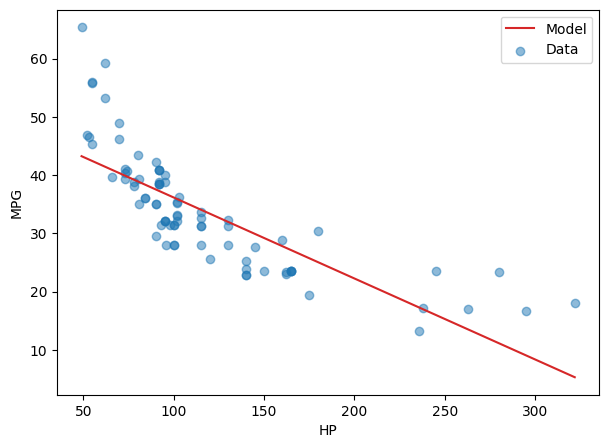
\includegraphics{../images/13-06a}
            \caption{Plot of the data with the fitted line from the linear model.}
          \end{figure}
    \item
          \inputminted{python}{../code/ex13_06b.py}
          \inputminted{text}{../output/ex13_06b.txt}

          \begin{figure}[H]
            \centering
            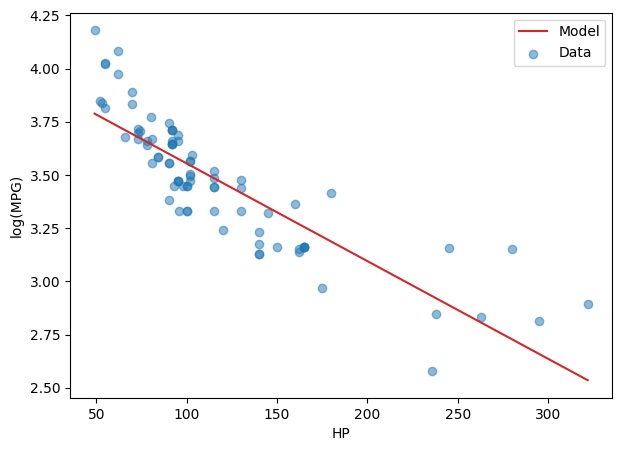
\includegraphics{../images/13-06b}
            \caption{Plot of the $\log(\text{MPG})$ response data with the
              fitted line from the linear model.}
          \end{figure}

          A linear model seems to fit the $\log(\text{MPG})$ response data
          better than then original $\text{MPG}$ response.
  \end{enumerate}
\end{ex}

\begin{ex}
  \begin{enumerate}[(a)]
    \item~
          \inputminted{python}{../code/ex13_07a.py}
          \inputminted{text}{../output/ex13_07a.txt}
    \item
          \inputminted{python}{../code/ex13_07b.py}
          \inputminted{text}{../output/ex13_07b.txt}
    \item
          \inputminted{python}{../code/ex13_07c.py}
          \inputminted{text}{../output/ex13_07c.txt}
    \item
          \inputminted{python}{../code/ex13_07d.py}
          \inputminted{text}{../output/ex13_07d.txt}
  \end{enumerate}
\end{ex}

\begin{ex}
  Let $Y=X\beta+\epsilon$. Suppose that $\epsilon_i\,|\,X_i\sim N(0,\sigma^2)$,
  and note that then by an identical argument to Section 13.2,
  \[
    \ell_S
    =-n\log{\sigma}
    -\frac{1}{2\sigma^2}\sum_{i=1}^n\left(Y_i-X_i\beta\right)^2.
  \]
  We then have
  \begin{align*}
    -2\sigma^2(\ell_S-|S|)-2n\sigma^2\log{\sigma}
     & =-2\sigma^2\left(
    -n\log{\sigma}-\frac{1}{2\sigma^2}\sum_{i=1}^n\left(Y_i-X_i\beta\right)^2-|S|
    \right)-2n\sigma^2\log{\sigma}                                                              \\
     & =\sum_{i=1}^n(Y_i-X_i\beta)^2+2|S|\sigma^2+2n\sigma^2\log{\sigma}-2n\sigma^2\log{\sigma} \\
     & =\Rtr+2|S|\sigma^2,
  \end{align*}
  i.e.\ Mallow's $C_p$ statistic is equal to a negative constant times AIC plus
  a constant. Therefore, maximizing AIC is equivalent to minimizing Mallow's
  $C_p$.
\end{ex}

\begin{ex}
  \begin{enumerate}[(a)]
    \item We have
          \begin{align*}
            \P{J_n=0}
             & =\P{AIC_0 > AIC_1}                                                           \\
             & =\P{\ell(0) > \ell(\thetahat)-1}                                             \\
             & =\P{-\frac{1}{2}\sum_{i=1}^nX_i^2 > -\frac{1}{2}\sum_{i=1}^n(X_i-\Xbar)^2-1} \\
             & =\P{\sum_{i=1}^nX_i^2-\sum_{i=1}^n(X_i-\Xbar)^2 < 2}                         \\
             & =\P{\sum_{i=1}^n\left[X_i^2-X_i^2+2X_i\Xbar-\Xbar^2 \right] < 2}             \\
             & =\P{n\Xbar^2 < 2}.
          \end{align*}
          If $\mathcal{M}_0$ is the true model, i.e.\ $\theta=0$, we have
          \[
            \P{J_n=0}
            =\P{|\sqrt{n}\Xbar| < \sqrt{2}}
            =\Phi(\sqrt{2})-\Phi(-\sqrt{2})
            \approx 0.8427.
          \]
          Otherwise,
          \begin{align*}
            \P{J_n=0}
             & =\P{n\Xbar^2 < 2}                                                                \\
             & =\P{-\sqrt{\frac{2}{n}} < \Xbar < \sqrt{\frac{2}{n}}}                            \\
             & =\P{-\sqrt{\frac{2}{n}}-\theta < \Xbar-\theta < \sqrt{\frac{2}{n}}-\theta}       \\
             & =\P{-\sqrt{2}-\sqrt{n}\theta < \sqrt{n}(\Xbar-\theta) < \sqrt{2}-\sqrt{n}\theta} \\
             & =\Phi(\sqrt{2}-\sqrt{n}\theta)-\Phi(-\sqrt{2}-\sqrt{n}\theta),
          \end{align*}
          and therefore
          \[
            \lim_{n\to\infty}\P{J_n=0}
            =\lim_{n\to\infty}\left[\Phi(\sqrt{2}-\sqrt{n}\theta)-\Phi(-\sqrt{2}-\sqrt{n}\theta)\right]
            =0.
          \]
    \item We proved earlier that assuming $\theta\neq 0$,
          $\widehat{f}_n\xrightarrow{P}\phi_{\thetahat}$. Note that
          \begin{align*}
            D(\phi_\theta, \phi_{\thetahat})
             & =\int \frac{1}{\sqrt{2\pi}}\exp\left\{-\frac{(x-\theta)^2}{2}\right\}
            \log\left(\frac{\frac{1}{\sqrt{2\pi}}\exp\left\{-\frac{(x-\theta)^2}{2}\right\}}{\frac{1}{\sqrt{2\pi}}\exp\left\{-\frac{(x-\thetahat)^2}{2} \right\}}\right)\,\d{x} \\
             & =\int \frac{1}{\sqrt{2\pi}}\exp\left\{-\frac{(x-\theta)^2}{2}\right\}
            \left(\frac{(x-\thetahat)^2}{2}-\frac{(x-\theta)^2}{2}\right)\,\d{x}                                                                                                \\
             & =\frac{1}{2}\int \frac{1}{\sqrt{2\pi}}\exp\left\{-\frac{(x-\theta)^2}{2}\right\}
            \left((\thetahat^2-\theta^2)-2x(\thetahat-\theta)\right)\,\d{x}                                                                                                     \\
             & =\frac{\thetahat^2-\theta^2}{2}-\theta(\thetahat-\theta)                                                                                                         \\\
             & =\frac{1}{2}(\thetahat-\theta)^2,
          \end{align*}
          which converges in probability to $0$ since $\thetahat-\theta$
          converges in probability to $0$.
    \item We have
          \begin{align*}
            \P{J_n=0}
             & =\P{BIC_0 > BIC_1}                                                                            \\
             & =\P{\ell(0) > \ell(\thetahat)-\frac{1}{2}\log{n}}                                             \\
             & =\P{-\frac{1}{2}\sum_{i=1}^nX_i^2 > -\frac{1}{2}\sum_{i=1}^n(X_i-\Xbar)^2-\frac{1}{2}\log{n}} \\
             & =\P{\sum_{i=1}^nX_i^2-\sum_{i=1}^n(X_i-\Xbar)^2 < \log{n}}                                    \\
             & =\P{\sum_{i=1}^n\left[X_i^2-X_i^2+2X_i\Xbar-\Xbar^2 \right] < \log{n}}                        \\
             & =\P{-\sqrt{\frac{\log{n}}{n}}<\Xbar < \sqrt{\frac{\log{n}}{n}}}                               \\
             & =\P{-\sqrt{\log{n}}-\sqrt{n}\theta <\sqrt{n}(\Xbar-\theta) < \sqrt{\log{n}}-\sqrt{n}\theta}.
          \end{align*}
          Assuming the true model is $\theta=0$,
          \begin{align*}
            \lim_{n\to\infty}\P{J_n=0}
             & =\lim_{n\to\infty}\P{-\sqrt{\log{n}}<\sqrt{n}\Xbar < \sqrt{\log{n}}}          \\
             & =\lim_{n\to\infty}\Phi(\sqrt{\log{n}})-\lim_{n\to\infty}\Phi(-\sqrt{\log{n}}) \\
             & =0,
          \end{align*}
          while if $\theta\neq 0$,
          \begin{align*}
            \lim_{n\to\infty}\P{J_n=0}
             & =\lim_{n\to\infty}\Phi(\sqrt{\log{n}}-\sqrt{n}\theta)
            -\lim_{n\to\infty}\Phi(-\sqrt{\log{n}}-\sqrt{n}\theta)
            =0.
          \end{align*}
  \end{enumerate}
\end{ex}

% 10
\begin{ex}
  \begin{enumerate}[(a)]
    \item Note that
          \[
            \P{\Yhat_*-2s < Y_* < \Yhat_*+2s}
            =\P{-2 < \frac{Y_*-\Yhat_*}{s} < 2},
          \]
          where $\var{Y_*-\Yhat_*}=\var{\epsilon}+\var{\Yhat_*}=\sigma^2+s^2$
          and $\E{Y_*-\Yhat_*}=0$. Therefore,
          \[
            \frac{Y_*-\Yhat_*}{s}\approx N\left(0, 1+\frac{\sigma^2}{s^2}\right),
          \]
          and thus
          \[
            \P{-2 < \frac{Y_*-\Yhat_*}{s} < 2}\neq 0.95.
          \]
    \item We have
          \begin{align*}
            \var{Y_*-\Yhat_*}
             & =\var{Y_*-\Yhat_*}                                                                     \\
             & =\var{\beta_0+\beta_1X_*+\epsilon-\betahat_0-\betahat_1X_*}                            \\
             & =\var{\betahat_0+\betahat_1X_*}+\var{\epsilon}                                         \\
             & =\var{\betahat_0}+X_*^2\var{\betahat_1}+2X_*\cov{\betahat_0,\betahat_1}+\var{\epsilon} \\
             & =\frac{\sigma^2}{n^2s_X^2}
            \sum_{i=1}^n\left(X_i^2-2X_*X_i+X_*^2
            \right)+\sigma^2                                                                          \\
             & =\left[\frac{\sum_{i=1}^n(X_i-X_*)^2}{n\sum_{i=1}^n(X_i-\Xbar)^2}+1\right]\sigma^2     \\
             & =\xi_n^2,
          \end{align*}
          and therefore,
          \begin{align*}
            \P{\Yhat_*-2\widehat{\xi}_n < Y_* < \Yhat_*+2\widehat{\xi}_n}
             & =\P{-2 < \frac{Y_*-\Yhat_*}{\widehat{\xi}_n} < 2} \\
             & \approx \P{-2 < N(0,1) < 2}                       \\
             & \approx 0.95.
          \end{align*}
  \end{enumerate}
\end{ex}

\begin{ex}~
  \inputminted{python}{../code/ex13_11.py}
  \inputminted{text}{../output/ex13_11.txt}
\end{ex}